%% Capitolul 0: INTRODUCERE
%%
%%

\addcontentsline{toc}{chapter}{Introducere}
\markboth{\bf Introducere}{\bf Introducere}

\chapter*{Introducere}
\label{capintro}
\markboth{\bf Introducere}{\bf Introducere}

@Inv@a@tarea automat@a a devenit un subiect de interes din ce @in ce mai important, aceast@a fiind utilizat@a @in vaste domenii, precum: industria auto, alimentar@a, agricol@a, bancar@a, aerospa@tial@a @si mai cu seam@a @in industria tehnologiei informa@tiei. Unul din rolurile ei cele mai importante const@a @in analiza @si clasificarea datelor, predic@tia unor evenimente @in baza unor fapte deja @int@amplate, crearea unui profil virtual pentru un grup de utilizatori, etc.


Datorit@a marei conectivit@a@ti dintre oamenii din ziua de ast@azi; sistemele politice, economice @si rela@tiile interumane au devenit extrem de complexe. Totul a devenit interconectat. O ideea a unui singur individ poate fi transmis@a pe tot globul p@am@antesc, aceasta idee putand afect\^ and milioane de oameni \^ in diverse locuri @si a c\^ arui impact politic @si economic poate fi greu de estimat. De asemenea, un incident economic local, un dezastru natural, sau un conflic politic dintre dou@a @t@ari pot avea efecte devastatoare asupra economiei globale @si a structurii geopolitice curente.

Fiecare eveniment din ziua de ast@azi are o influen@t@a mai mic@a sau mai mare aupra acestei mari re@tele de sisteme ale civiliza@tiei umane. @Intrebarea natural@a la aceast@a dilemna este: putem face o estimare aupra acestor evenimente @si ale cazurilor lor speciale? Se poate, @si asta datorit@a faptului ca multe evenimente sunt monitorizate @si @inregistrate, precum: tranzac@tiile bancare, documente legislative @si juridice, vremea, traseele @si destina@tiile ma@sin@ariilor de transport marf@a (automobile, avioane, vapoare), discursuri @si opinii @in re@tele sociale, date medicale din dispozitive inteligente (telefoane smart, ceasuri @si br@atari smart), date provenite din simul@ari virtuale sau experimente. 

Tot acest mare volum de informa@tii @si metodele de manipulare, stocare @intr@a @in a@sa numita categorie {\sl Big Data}. Analiz@a acestui volum imens de date devine o sarcin@a foarte dificil@a @si laborioas@a @in cazul metodelor conven@tionale de analiz@a a datelor folosind statistic@a clasic@a. @In esen@t@a, @inv@a@tarea automat@a se foloseste at@at de teoria clasic@a c\^  at @si de noile descoperiri @in calculul numeric pentru a crea modele matematice dinamice care pot acumula cuno@tin@te @si ac@tiona @in baza lor folosind toate datele pe care le prime@ste ca set de @inv@a@tare.

\^ In aceast\u a lucrare se va analiza cum algoritmii de @inv@a@tare automat@a  pot fi folosi@ti @in crearea unui agent autonom care s@a @indeplineasc@a sarcinii @intr-un spa@tiu 2-dimensional. Problema const@a @in rezolvarea unui traseu de tip matrice @in care agentul trebuie s@a ajung@a la destina@tie f@ar@a a produce un accident.

Analiza se va face cu ajutorul unei aplica@tii web interactive @in care vom simula mediul nostru 2-dimensional reprezentat de un labirint @si care ne va permite analiza datelor furnizate de c@atre agent @in timpul sesiuni de antrenament pentru determinarea eficien@tei @si fiabilit@a@tii algoritmilor.


\hspace{0.2cm}

@In primul capitol este descris termenul de @inv@a@tare automat@a, care sunt subdomeniile sale, cum este folosit @in @industire. 

@In al doilea capitol este o mic@a introducere pentru re@telele neuronale artificiale.

@In al treilea capitol vor fi prezenta@ti c@a@tiva algoritmi de @inv@a@tare, iar al patrulea descrierea aplica@tiei.

@In al patrulea capitol se va descrie structura aplica@tiei web, a componentelor sale @si modul cum acestea interac@tioneaz@a.

\newpage

%%CAPITOLUL 1
%%
%%
\chapter{ @Inv@a@tare automat@a }
\index{@Inv@a@tare automat@a}

\section{Istoric}
\index{sectiune!S1.1}

	@Inv@a@tarea automat@a este o ramur@a a @inteligen@tei artificiale care se ocup@a cu studiul tehnicilor @si metodelor prin care se ofer@a unui calculator abilitatea de a @inv@a@ta. Prin @inv@a@tare ne referim la posibilitatea de a oferii o decizie @in baza unor cuno@stin@te deduse din experien@te anterioare.

 Multe tehnici din @inv@a@tarea automat@a au la baz@a modelul de interac@tiune al neuronilor, descris de c@atre Donal Hebb @in cartea sa {\sl The Organization of Behavior} \cite{donald-hebb-book}. Termenul de @inv@a@tare automat@a (@in englez@a {\sl machine learning}) a aparut @in anul 1953, dat de Arthur Samuel, creatorul unui program de jucat checker, capabil s@a ia decizii bazate pe experien@tele anterioare \cite{arthur-samuel}. @In anul 1957, Frank Rosenblatt creaz@a Perceptron-ul - utilizat @in crearea unui calculatorul capabil s@a recunoasc@a forme @intr-o imagine - folosindu-se de observa@tiile din lucr@arile lui Donald Hebb @si Arthur Samuel. Perceptron-ul de unul singur are o putere destul de limitat@a, dar odat@a cu descoperirea utiliz@arii sale @in combina@tii de mai multe straturi a dat na@stere la termenul de re@tea neuronal@a. 
 
 De-a lungul timpului, acest domeniu a avut o evolu@tie @inceat@a, un factor important find capabilit@a@tile limitate de procesarea ale calculatoarelor. Dar odat@a cu avansurile tehnologice, cercetarea @in acest domeniu a @inceput s@a fie din ce @in ce mai activ@a, @in ultimii ani culmin\^ and cu evenimente care au atras interesului publicului general, precum: IBM's Deep Blue, IBM's Watson, Google's Deepmind @si Google's AlphaGo.
 
 
\newpage

\section{Clasificare}

Fiind un domeniu foarte vast @si cuprinz@tor, aceasta se @imparte @in 3 mari categorii:
\hspace{0.2cm}\begin{itemize}
	\item @Inv@a@tare supervizat@a
	\item @Inv@a@tare nesupervizat@a
	\item @Inv@a@tare prin recompens@a
\end{itemize}

\vspace{0.3cm}
@In @inv@a@tarea supervizat@a, procesul de antrenare se bazeaz@a pe analiza unor date formate din perechi de valori intrare-ie@sire (set de date etichetat) pentru calibrarea func@tiilor de deducere. Este folosit pentru rezolvarea problemelor de clasificare.

Exemple de algoritmi:
\begin{itemize}
	\item Support-vector machines
	\item Regresia liniar@a
	\item Regresia logistic@a
	\item Arbori de decizie
	\item Re@tele neuronale
	\item Clasificator bayesian naiv
\end{itemize}

Pentru @inv@atarea nesupervizat@a, procesul de antrenare const@a @in crearea unor modele interne de recunoa@stere a unor tipare @in urma analizei unui set de date neetichetat. Este deseori folosit @in descoperirea similarit@a@tilor @si diferen@telor @intr-un set de date.

Exemple de algoritmi:
\begin{itemize}
	\item K-means clustering
	\item Autoencoders
	\item Analiza componentei principale
	\item Descompunerea valorilor singulare
\end{itemize}

@In @inv@a@tarea prin recompens@a, procesul de antrenare const@a @in maximizarea unei func@tii de recompens@a, modelul calibr@andu-se astfel @incat deciziile luate s@a duc@a spre ob@tinerea unei recompense c\^ at mai mari.

Exemple de algoritmi:
\begin{itemize}
	\item Monte Carlo
	\item Q-learning
	\item SARSA
	\item Deep Q Network
	\item Proximal Policy Optimization
	\item Deep Deterministic Policy Gradient
	\item Trust Region Policy Optimization
\end{itemize}

\section{Industrie}

	Tot mai multe aplica@tii folosesc tehnici de @inv@a@tare automat@a pentru optimizarea produselor, servicilor @si interac@tiunilor cu utilizatorii. Cele mai notabile utiliz@ari fiind:
\begin{itemize}
	\item Algoritimi de c@autare a @stirilor @in baza unor preferin@te oferite explicit sau implicit de catre utilizator.
	\item Reclame personalizate generate dup@a profilele utilizatorilor.
	\item Sisteme de recomand@ari produse.
	\item Etichetarea obiectelor sau persoanelor @in imagini, @inregistr@ari audio sau video.
	\item Sisteme robotice autonome.
	\item Ma@sini autonome.
	\item Sisteme meteorologice
	\item Sisteme de detectare a fraudelor @intr-un sistem bancar.
	\item Clasificare @si predic@tia evenimentelor. 
	\item Optimizarea proceselor de produc@tie a m@arfurilor.
	\item Optimizarea procesului de antrenare pentru atle@ti.
\end{itemize}

	Companiile sunt foarte interesate de modul cum interac@tioneaz@a @si percep clien@tii produselor lor, ele @incerc\^ and mereu s@a colecteze informa@tii pentru despre modul cum sunt utilizate produsele @in activitatea utilizatorului. Aceste campanii de colectare a datelor a devenit din ce @in ce mai agresiv@a, marile companii software specializate @in re@tele sociale (Facebook, Twitter, Youtube, Linkedin, Reddit) v@and datele utilizatorilor @in vederea oferirii unui profil al consumatorului pentru a stabili interesul pentru produs. 
	 
\section{Programe software pentru dezvoltare}

Interesul puternic pentru acest domeniu a venit @in principal din partea marilor companii software @si hardware, ele dezvolt@and puternice biblioteci pentru procesarea datelor, crearea de re@tele neuronale, algoritmi de @inv@a@tare, etc. Pentru sprijinirea domeniului, aceste unelte sunt oferite dupa ca aplica@tii cu surs@a deschis@a ( @in englez@a {\sl open source} ), av@and o licen@t@a deseori foarte permisibil@a @in vederea utiliz@ari personale @si comerciale.

Calitatea acestor unelte le-a f@acut s@a devin@a un standard @in industrie, at@at comercial@a c\^ at @si academic@a.

Example de biblioteci sau aplica@tii software:

\begin{itemize}
	\item Tensorflow - bibliotec@a dezvoltat@a de c@atre Google @in vederea utiliz@ari cu usurin@t@ a algoritmilor de @inv@a@tare, c@at @si func@tii utilitare pentru manipularea datelor.
	\item PyTorch - bibliotec@a dezvoltat@a de c@atre Facebook pentru protiparea aplica@tilor de viziune computerizate, procesarea limbajului natural, etc.
	\item ML.NET - bibliotec@a dezvoltat@a de Microsoft pentru crearea rapid@a a unor aplica@tii de procesare a datelor folosind algoritmi de @inv@a@tare.
	\item scikit-Learn - bibliotec@a care con@tine func@tii statistice folosite pentru analiza datelor.
	\item Apache Spark - bibliotec@a de aplica@tii destinate pentru procesarea unui volum foarte mare de date.
	\item Apache Kafka - aplica@tie care permite stocarea @si distribuirea unui volum foarte mare de date @in timp real c@atre mai mul@ti consumatori.
	\item Caffe - bibliotec@a pentru dezvoltare aplica@tilor pentru medii de lucru care nu dispun de o putere de procesare foarte mare, precum dispozitivele mobile.
	\item Keras - bibliotec@a pentru dezvoltarea re@telelor neuronale
	\item H2O.ai - platform@a de procesare @si analiz@a a datelor pentru mediul comercial
	
\end{itemize}

\section{Big Data}

O component@a esen@tial@a pentru @inv@a@tarea automat@a este gestionarea datelor care vor fi folosite @si produse de c@atre algoritmi algoritmii @inv@a@tare. Aceast@a gestionare a informa@tiilor, de cele mai multe ori, va intra @in cadrul domeniului de {\sl Big Data }

Conform Uniunii Europene: ,,Big data se refer@a la volume de date colectate at\^ at de mari @si complexe @inc\^ at este nevoie de noi tehnologii, cum ar fi inteligen@t@a artificial@a, pentru a le procesa. Datele provin din nenum@arate surse diferite.''\cite{eu-big-data-definition}

Volumul de date pe care omenirea @il produce cre@ste de la an la an, cea ce face  analiza @si intelegerea datelor s@a fie o sarcin@a din ce @in ce mai dificil@a. Tot mai mul@ti oameni @incep s@a aib@a acces la internet, iar num@arul de dispozitive inteligente (smart phone, smart watch, smarth TV) pe care un individ de dispune cre@ste odat@a cu avansul tehnologic.

Principalele surse de provenien@t@a ale acestor date sunt:
\begin{itemize}
	\item Re@tele sociale - mesaje, imagini create de utilizatori pentru a@si exprima opinia la situa@tia sociala, economic@a @si politic@a - datele pot fi utilizate pentru stabilirea unor tendin@te sociale cu privire la activitatea @si starea emo@tional@a curent@a @si viitoare a oamenilor.
	\item Mediul @si natura - date provenite de la sateli@ti @si senzori pentru monitorizarea schimb@arilor climatice - folosite pentru predic@tia posibilelor dezastre naturale cauzate de activit@a@tile omului.
	\item Sector public - documente, certificate, atestate, adeverin@te emise de c@atre institu@tile publice - pot fi utilizate @in eficientizarea servicilor publice.
	\item Transport - date colectate prin GPS @si de la diferi@ti operatori @in domeniul transportului (transportul public, aeroporturi, g@ari) - pentru optimizarea rutelor @si a curselor de transport.
	\item Sector Medical - fi@se medicale ale pacien@tilor - monitorizarea st@arii de s@anatatea a cet@a@teinolor, utile pentru detectarea posibilelor amen@t@ari de tip biologic.
	\item Iternetul Lucrurilor ({\sl Internet of Things}) - date provenite de la diverse aparate, precum: telefon, ceas, televizor, senzor de gaz, sensor de umiditate, camere video, etc. - utilizate la monitorizare activit@a@tii invidului cu scopul de a u@sura anumite sarcini sau pentru a prevenii incidente.
	\item Sector industrial - re@tele industriale de comunica@tii ( senzori, magistrale de teren, re@tele celulare), rapoarte economice - folosite pentru automatizare @si @imbun@at@a@tirea produselor @si a servicilor. 
	\item Sector bancar - tranzac@tii financiare, rapoarte - utilizate pentru detectarea fraudelor bancare, stabilirea ratelor la dob@anzi, @imprumuturi, schimb valutar, etc.
\end{itemize}

Toate aceste benificii sunt importante pentru societatea din ziua de ast@azi, companii mare concureaza pentru crearea de infrastructur@a @si servicii pentru stocarea @si examinarea datelor.

Exemple de servicii:

\begin{itemize}
	\item Amazon Web Services - cel mai mare furnizor de servicii @si infrastructur@a cloud din lume (av\^ and peste 200 de solu@tii software).
	\item Microsoft Azure 
	\item Google Cloud Platform
	\item IBM Cloud
	\item Oracle Cloud
	\item Alibaba Cloud
\end{itemize}

	
%%CAPITOLUL 2
%%
%%

\chapter{Re@tele neuronale artificiale}

\index{capitol!C2}
\index{@Inv@a@tare automat@a}

\section{Introducere}

O re@tea neuronal@a artificial@a este un model computa@tional inspirat din structura @si modul de fun@tionare al creierului biologic. Conexiunile dintre neuronii artificiali se asem\^ an@a sinapselor, fiecare neuron se conecteaz@a cu alt neuron prin intermediul unor muchii. Semnalul trimis prin aceste muchii este ponderat de ni@ste parametri numi@ti ponderi sinaptice. Mai mul@ti neuroni grupa@ti formeaza un strat, iar mai multe straturi formeaz@a o re@tea.

Procesul de @inv@a@tare presupune g@asirea unor valori potrivite pentru ponderile sinaptice astfel @inc\^ at procesarea semnalului de intrare s@a ofere rezultatul dorit.


\section{Structur@a}

Structura principal@a al unui neuron artificial este bazat pe modelul Perceptron-ului al lui Donald Hebb, modelul matematic fiind:

$$
	y = \varphi \left( \sum_{k=1}^{n} w_k * x_k + b \right)
$$

,unde $x$ este vectorul de intrare ({\sl input vector}), $y$ vectorul de ie@sire ({\sl output vector}), $w$ ponderea sinaptic@a ({\sl weight}), $b$ deplasarea ({\sl bias}) @si $\varphi$ este func@tia de activare sau transfer ({\sl activation function}).

Vectorul de intrare este format din numerele reale, aceste numere put\^ and reprezenta: imagini, frecven@te, etichete codificate, valori provenite din senzori, etc. Ponderile sinaptice au rolul de a cre@ste sau descreste puterea semnalul reprezentat de valorile vectorului de intrare. Func@tia de activare preia semnalul ponderat @si ofer@a o valoarea spefic@a @in baza acestuia. Deplasarea ajut@a la deplasarea semnalului ponderat pentru o mai bun@a aproximare necesar@a pentru @indeplirea anumitor condi@tii ale func@tiei de activare.

\begin{exemplu}

	Un neuron artificial care ac@tioneaz@a precum o poarta logic@a {\bf SAU}(OR) pentru dou@a numere binare are forma:
$$
	y = \varphi ( x_1 + x_2 - 0.5 )
$$
,unde $x = \{ x_i | x_i \in \{0, 1\} \}$, $y \in \{0, 1\}$, $w_1 = 1$, $w_2 = 1$,$b = -0.5$, iar func@tia de activare este: 
$$
	\varphi ( u ) = \left\lbrace
		\begin{array}{lc}
			1 & u \geq 0 \\
			0 & u < 0
		\end{array}
	\right.
$$
\end{exemplu}

{\bf Verificare}. Pentru $x = [1, 0]$, avem $u = 1 + 0 - 0.5 = 0.5$ @si $y = \varphi(u) = \varphi(0.5) = 1$ (acela@si rezultat @si pentru $x = [0, 1]$ - datorit@a propieta@tii de comutativitate a adun@arii).
Pentru $x = [1, 1]$, avem $u = 1 + 1 - 0.5 = 1.5$ cu $\varphi (u) = \varphi ( 2 ) = 1$. Ultimul caz pentru $x = [0, 0]$, vom avea $u = 0 + 0 - 0.5 = -0.5$ cu $\varphi (-0.5) = 0$.

\begin{observatia}
	F@ar@a func@tia de activare, perceptronul ac@tioneaz@a precum o func@tie liniar@a. Prin utilizarea unei func@tii de activare potrivite, puteam aborda mai u@sor problemele neliniare, precum cele pentru clasificarea datelor @in diverse categorii.
\end{observatia}

Un singur perceptron ofer@a doar o singur@a valoare de ie@sire. Dac@a dorim s@a avem mai multe valori de ie@siri trebuie s@a mai adaug@am perceptroni. Gruparea de neuroni artificiali se nume@ste {\sl strat}.

Structura unui strat format din perceptroni arat@a astfel @in form@a matriceal@a:

$$
	\begin{bmatrix}
		u_1 \\
		u_2 \\
		\vdots \\ 
		u_n \\
	\end{bmatrix}	
	= 
	\begin{bmatrix}
		w_{11} & w_{12} & \cdots & w_{1n} \\
		w_{21} & w_{22} & \cdots & w_{2n} \\
		\cdots & \cdots & \cdots & \cdots \\
		w_{n1} & w_{n2} & \cdots & w_{nn} \\
	\end{bmatrix}
	\begin{bmatrix}
		x_1 \\
		x_2 \\
		\vdots \\
		x_n \\
	\end{bmatrix}
	+
	\begin{bmatrix}
		b_1 \\
		b_2 \\
		\vdots \\
		b_n
	\end{bmatrix}
$$

$$
\begin{bmatrix}
		y_1 \\
		y_2 \\
		\vdots \\ 
		y_n \\
	\end{bmatrix}	
	=
	\begin{bmatrix}
		\varphi (u_1)\\
		\varphi	(u_2) \\
		\vdots \\
		\varphi (u_n)
	\end{bmatrix}
$$

Rezultatele acestui strat pot fi transmise c@atre un alt strat care poate avea o alt@a func@tie de activare, astfel putem crea modele matematice mai complexe. Aceast@a @in@siruire de straturi se nume@ste {\sl re@tea}. Straturile intermediare sunt deseori referite ca {\sl straturi ascunse}. Iar o re@tea cu foarte multe straturi asunse poart@a denumirea de {\sl profund@a (deep)}.

Re@tele pot fi structurate @si sub forma unui graf. Fiecare neuron find repezentat de un nod, iar muchiile grafului sunt conexiunile dintre neuroni. Dac@a graful suport nu con@tine cicluri, spunem c@a este uni-directional - o denumire uzual@a peste acest tip de re@tea este {\sl feed-forward (FF)} (denumire pe care o vom folosii @si @in restul acestei lucr@ari). De asemenea, neuroni pot fi interconecta@ti (graful suport con@tine cicluri), fapt care poate oferii re@telei mai mult@a putere de modelare. Acest tip de re@tea este denumit @in general {\sl recurrent neural network (RNN)}

Re@telele neuronale artificiale pot fi considerate ca find "aproximatori universali"\cite{hornik-nn}: 
\begin{quotation}
	Re@telele feed-forward multistrat sunt,@in condi@tii generale ale func@tiei de activare ascuns@a, aproximatori universali dac@a dispun de un num@ar suficient de unit@a@ti asunse.
\end{quotation}

De-a lungul anilor, au fost create foarte multe tipuri de re@tele neuronale artificiale pentru a servii la rezolvarea de probleme din domenii dificile.

Exemple de tipuri de re@tele:

\begin{itemize}
	\item Feed Forward (FF)
	\item Deep Feed Forward (DFF)
	\item Radial Basis Network (RBF)
	\item Recurrent Neural Network (RNN)
	\item Long/Short Term Memory (LSTM)
	\item Markov Chain (MC)
	\item Deep Convolutional Network (DCN)
	\item Deconvolutional Network (DN)
	\item Support Vector Machine (SVM)
	\item Deep Belief Network (DBN)
\end{itemize}


\begin{figure}[h]
	\centering
	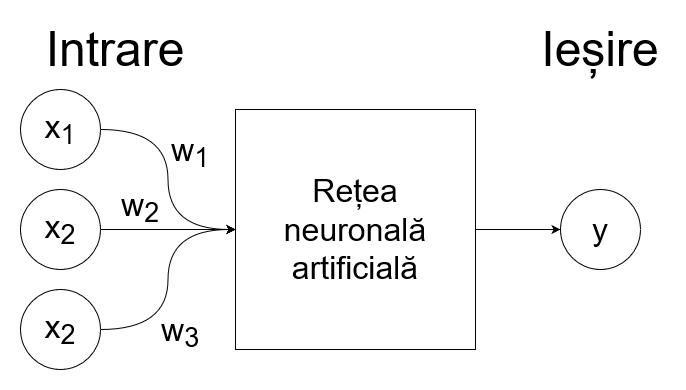
\includegraphics[scale=0.4]{nn_schema_1}
	\caption{Structura unei re@tele neuronale}
	\label{nn:schema}
\end{figure}




\section{Func@tii de activare @si metode de optimizare}
Func@tia de activare ajut@a re@teaua neuronal@a pentru @in@a@tarea de tipare complexe aflate @in setul de date analizat. Alegerea unei func@tii de activare este critic@a pentru performan@ta re@telei, @in special cazul problemelor neliniare.

Unele din cele mai folosite func@tii sunt:

$$
\begin{array}{rlcc}
	{\rm Identitate} & \varphi (x) &=& x \\
	{\rm Binary \, Step} & \varphi (x) &=& \left\lbrace
		\begin{array}{lc}
			1 & x \geq 0 \\
			0 & x < 0
		\end{array}
	\right. \\
	{\rm Logistic, Sigmoid} & \varphi (x) &=& \displaystyle\frac{1}{1 + e^{-x}} \\
	{\rm Rectified\, liniar\, unit (ReLU)}& \varphi (x) &=& \left\lbrace
		\begin{array}{lc}
			x & x \geq 0 \\
			0 & x < 0
		\end{array}
	\right. \\
	{\rm Softplus} & \varphi (x) &=& \ln ( 1 + e^x) \\
\end{array}
$$

Func@tiile de activare pot aproape orice func@tie liniar@a sau neliniar@a, dar unele  (precum cele enumerate anterior) ofer@a mai multe beneficii dec@at altele @in contextul antren@arii unei re@tele.

Crearea unei re@tele neuronale artificiale presupune alegerea tipurilor de straturi din care s@a fie compus@a @impreun@a cu func@tile lor de activare. La @inceput, ponderile sinaptice sunt de cele mai multe ori alese aleatoriu. Cea ce face ca aproximarea oferit@a de re@tea s@a nu una foarte bun@a.

Acest lucru duce la problema de optimizare a re@telei (g@asirea unor valori potrivite pentru ponderile sinaptice) astfel \^inc\^ at rezultatul aproxim@arii s@a fie unul satisf@ac\^ ator. Acest proces este referit uzual ca {\sl antrenare (training)}. Antrenarea este unul dintre cele mai dificile capitole al acestui domeniu, alegerea unui algoritm potrivit poate beneficii extraordinarea @in privin@ta g@asii unor valori optimale pentru ponderile sinaptice.

Re@telele neuronale artificiale folosite @in industrie (aplica@tii de recunoa@stere a obiectelor @in imagini; programe pentru traduceri, recunoa@steri de voce ) au o complexitate extrordinar@a at@at din punct de vedere al arhitecturii, care poate const@a dintr-un mix de diferite tipuri de re@tele, c\^ at @si al nivelului imens de date (de ordinul milioanelor de terabi@ti). Antrenarea acestora poate dura c\^ ateva zile sau c\^ ateva luni, @in cazuri rare fiind vorba de ani. A@sdar, un algoritm de optimizare eficient are un rol crucial @in acest proces.

\section{Tensorflow}
Tensorflow este o platform@a dedicat@a dezvolt@arii modelelor de @inv@a@tare automat@a. Acest@a a fost creat@a ini@tial de c@atre Google pentru a accelara dezvoltarea domeniului prin oferirea de programe ajut@atoare pentru crearea rapid@a a protipurilor. Datorit@a calit@atii superioare a programelor de prototipare @si a usurin@tei de utilizare, acesta a devenit o platform@a popular@a at\^ at @in mediul academic c\^ at @si industrial.

Datorit@a popularit@a@tii, platforma a beneficiat de multe contribu@tii importante din partea marilor companii din domeniul IT @si cel al semiconductoarelor, precum: PayPal, AMD, nVIDIA, Blomberg, Intel, IBM, Qualcomm, Uber, Arm, Twitter. De asemenea, platforma beneficieaza de medii interactive de @inv@a@tare, ideale pentru studen@ti sau profesioni@sti care doresc s@a dezvolte mici prototipuri de modele de @inv@a@tare automat@a.

Exemple de programe care fac parte din platforma Tensorflow:
\begin{itemize}
	\item Tensorflow Hub - biblioteca care g@azduie@ste modele predefinite create de comunitate, precum: modele pentru clasificare imaginilor, analiza limbajului natural, generatoare de imagini
	\item Model Optimization - programe dedicate optimiz@arii de modele
	\item TensorFlow Graphics - biblioteca care dispune de unelte pentru procesarea imaginilor
	\item TensorFlow Agents - biblioteca pentru dezolvatare agen@tilor @in cazul @Inv@a@tarii prin recompens@a
\end{itemize}

@In aceasta lucrare vom folosii aceste unelte pentru dezvoltarea unui model pentru agentul care va parcurge labirintul.

%%CAPITOLUL 3
%%
%%
\chapter{Metode de @inv@a@tare}
\index{capitol!C3}

\section{Lan@t @si proces Markov}

\index{lan@t Markov}
\index{process Markov}

La baza modelului de @inv@atare pe care il vom folosii @in atrenarea agentului stau princiipile fundamentale ale lan@tului Markov @si a procesului Markov.
Propietatea Markov afirm@a c@a viitorul depinde numai de prezent si nu de trecut. Un lan@t Markov este un model probabilistic care depinde numai de starea curenta pentru a prezice o stare viitoare. A@sadar, un lan@t Markov respect@a propietatea Markov.
Trecerea de la o stare la alta se nume@ste tranzi@tie, iar probabilitatea ei poart@a denumirea de probabilitate de tranzi@tie.

De cele mai multe ori, lan@tul Markov este reprezentat sub form@a de graf orientat al c@arui muchii reprezint@a probabilit@a@tile de tranzi@tie dintre varfuri. Suma probailit@a@tilor de tranzi@tie ale unui varf c@atre celelalte varfuri este mereu 1.

In cazul agentului nostru, dac@a ne-am imagina traseul ca find un lan@t Markov, atunci pozi@tiile din trase ar fi varfurile grafului, iar misc@arile agentului ar reprezenta muchiile. Putem asocia fiecarei mi@scare o probabilitate, iar parcurgerea grafului reprezint@a un posibil drum c@atre obiectiv.

A@sadar, dac@a ne-am dorii ca agentul s@a foloseasc@a aceasta idee pentru stabilirea unui drum pentru rezolvarea obiectivului trebuie s@a stabilim o strategie de parcurgere a grafului.
O strategie simpl@a ar fi una de tip {\sl Greddy}, @si anume agentul alege mereu ac@tiunea/muchia cu probabilitatea cea mai mare. Pentru ca aceasta strategie s@a aib@a succes trebuie ca valorile probabilit@atilor act@iunilor s@a conduc@a c@atre obiectiv @in urma parcugerii grafului.

Peste lan@tul Markov putem contrui un model matematic pentru modelarea procesului de decizie al agentului. Acest model con@tine urm@atoarele elemente:

\begin{itemize}
	\item Mul@timea st@arilor (S)
	\item Mul@timea ac@tiunilor (A)
	\item Probabilitatea de tranzi@tie dintr-o stare @in alta pentru o ac@tiune ($P_{s s^{\prime}}^a$)
	\item Probabilitatea de a primi o recompens@a @in urma tranzi@tiei ($R_{s s^{\prime}}^a$)
	\item Factor de atenuare, pondere care exprim@a importan@ta recompenselor imediate @si viitoare ($\gamma$)
\end{itemize}

Pentru a controla comportamentul agentului @in mediul de lucru, vom folosii un sistem de recompense pentru fiecare decizie luat@a. Dac@a dorim ca agentul sa evite anumite situa@tii precum luare de ac@tiuni care conduc la coliziuni cu anumite obiecte, vom asocia acestor decizii recompense negative. \^In contrast, dac@a dorim ca agentul s@a fac@a anumite ac@tiuni care duc la \^indeplinirea obiectivelor, acestor decizii li se vor asocia recompense pozitive.

A@sadar, dorim ca pe parcursul simul@arii agentul s@a acumuleze c\^ at mai multe recompense pozitive @si s@a sle evite pe c\^ at mai mult posibil pe cele negative. Acestu lucrul @il vom numi optimizare, iar procesul de antrenament implic@a modificarea re@telei neurale astfel @inc\^ cat ac@tiunile rezultate din datele de intrare s@a maximizeze recompensele acumulate.



\section{Ecua@tia Bellman}



\section{Q-Learning}

%%CAPITOLUL 4
%%
%%
\chapter{Aplica@tie}
\index{capitol!C3}

\section{Introducere}

Pentru aplica@tia @in care vom implementa algoritmit de @inv@a@tare ne dorim s@a avem disponibile urm@atoarele funct@ionalit@a@ti:

\begin{itemize}
	\item Vizualizare grafic@a pentru mediul simulat - Afi@sarea libirintului sub forma unei poze
	\item Grafice pentru analizelor datelor op@tiune din timpul sesiunilor de antrenament
	\item Elemente interactive care s@a ne permit@a modificare de parametri interni @in algoritmi
	\item Tabele care s@a afiseze informa@tii/date care urmeaz@a s@a fie procesate @si rezultatele acestora
\end{itemize}

Av\^ and @in vedere cerin@tele men@tionate anterior, platforma care ne poate permite @in o dezvoltare rapid@a asupra unei interfe@tei interactive foarte bogate este cea a aplicat@ilor destinate web-ului.

Pentru contruirea aplica@tiei vom folosii urm@atoare technologii:

\begin{itemize}
	\item Svelte - program pentru construirea aplica@tilor web care va reprezenta interfa@ta interactiv@a dedicat@a utilizatorului \cite{Svelte}
	\item Tensorflow.js - bibliotec@a dedicat@a pentru contruirea @si antrenarea re@telelor neuronale pentru aplica@tii web \cite{TensorflowJs}
	\item Echarts - bibliotec@a pentru contruirea de graficelor dedicate vizualizarii de date \cite{Echarts}
	\item Konva - bibliotec@a grafic@a pentru generarea imaginilor \cite{Konva}
\end{itemize} 

Elementele de baz@a vor fi construite folosind Svelte, acestea find: butoane, c@ampuri de introducere a datelor, tabele pentru prezentarea informa@tiilor, containere pentru pozi@tionare. Construirea labirintului se va face prin intermediul lui Konva, care ne permite @si modificare rapid@a a imaginii @in func@tie de starea intern@a a simulatorului. Datele provenite din sesiunile de antrenament for fi afi@sate imediat dup@a fiecare sesiune cu ajutorul graficelor generate de Echarts.

Algoritmii de @inv@a@tare vor fi construi@ti folosind func@tile oferite de c@atre Tensorflow, aceastea oferind urm@atoarele capabilit@ati: crearea de straturi cu diverse func@tionalit@a@ti, func@tii de activare, algoritimi de optimizare, metode utilitare de salvare @si de creare a unor modele secven@tiale formate din mai multe straturi de neuroni.

\section{Structur@a}





Labirintul este de forma unei matrici, fiecare celul@a @indepline@ste un anumit rol: drum, obstacol, ie@sire, etc. Clasa principala dedicat@a definirii structurii de reprezentare a la\-bi\-rin\-tului este denumit@a \textbf{Board}. Aceast@a clas@a define@ste mediul simulat @si intereac@tiunile disponibile pentru agent.

Pentru codificare vom avea urm@atoarele reguli: spa@tiul liber va avea cifra 1, un obstacol cifra 2, iar pentru ie@sire cifra 3. Pentru pozi@tile agentului, la codificarea celulei de matrice se va adauga prefixul 1. Exemple de definiri al mediului simulat prin codificare se pot observa @in tabelul~\ref{tab:codific-lab}.


\begin{table}[h]
	\begin{center}
		\begin{tabular}{ccccc}
			\begin{tabular}{|c|c|c|}
				\hline
				11 & 1 & 2 \\
				\hline
				1 & 2 & 2 \\
				\hline
				1 & 1 & 3 \\
				\hline
			\end{tabular} & 
			\begin{tabular}{|c|c|c|}
				\hline
				1 & 1 & 2 \\
				\hline
				11 & 2 & 2 \\
				\hline
				1 & 1 & 3 \\
				\hline
			\end{tabular} &
			\begin{tabular}{|c|c|c|}
				\hline
				1 & 1 & 2 \\
				\hline
				1 & 2 & 2 \\
				\hline
				11 & 1 & 3 \\
				\hline
			\end{tabular} &
			\begin{tabular}{|c|c|c|}
				\hline
				1 & 1 & 2 \\
				\hline
				1 & 2 & 2 \\
				\hline
				1 & 11 & 3 \\
				\hline
			\end{tabular} &
			\begin{tabular}{|c|c|c|}
				\hline
				1 & 1 & 2 \\
				\hline
				1 & 2 & 2 \\
				\hline
				1 & 1 & 13 \\
				\hline
			\end{tabular} \\
		\end{tabular}
	\end{center}
	\caption{Exemple de codific@ari ale structurii labirintului}
	\label{tab:codific-lab}
\end{table}

Sunt disponibile patru ac@tiuni pe care agentul poate s@a le ia: sus, jos, st\^ anga @si dreapta. Ca o ac@tiune s@a fie valid@a, aceasta trebuie s@a @indeplineasc@a urm@atoarea condi@tie: ac@tiunea nu trebuie s@a fac@a agentul s@a ias@a din labirint atunci c\^ and se afl@a la margine. Dac@a se @int\^ ampl@a aces lucru, clasa {\bf Board} va pastra pozi@tia agentului @si va transmitele faptul c@a mutare este invalid@a celorlalte componente astfel @inc\^ at acestea s@a poat@a stabili o recompens@a astfel @inc\^ at ca pe viitor agentul s@a evite astfel de situa@tii.

Reprezentarea libirintului sub form@a de imagine este dat@a de clasa \textbf{BoardUI}. Aceasta are rolul s@a creeze reprezentarea vizual@a a labirintului folosind datele furnizate de c\^ atre clasa \textbf{Board}. Aceast@a reprezentare poate fi observat@a @in figura \ref{fig:labirint-imagine}. Agentul este prezentat sub forma unui cerc albastru, spa@tiul liber sub forma unui p@atrat gri, iar obiectivul cu un p@atrat violet.

\begin{figure}[h]
	\centering
	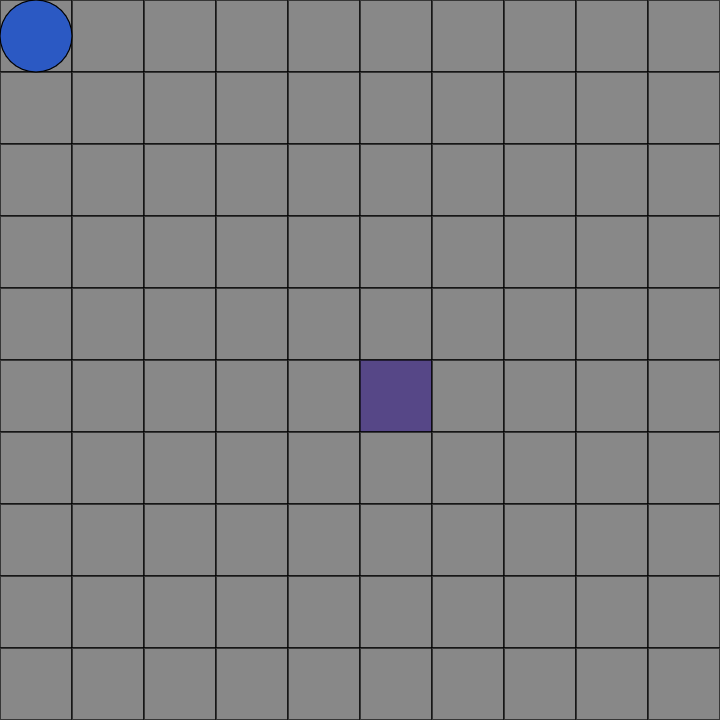
\includegraphics[scale=0.25]{app-labirint-imagine}
	\caption{Reprezentarea vizual@a a labirintului @in starea ini@tial@a}
	\label{fig:labirint-imagine}
\end{figure}

Clas@a \textbf{BoardUI} este legat@a de clasa \textbf{Board} printr-un sistem reactiv de notificare, astfel @inc\^ at orice schimbare care duce la modificarea st@arii labirintului (exemplu: miscarea agentului ) se propaga imediat c\^ atre aceasta, astfel imaginea este modificat@a imediat cu noile date (figura \ref{fig:labirint-imagine-cu-mutare}).

Toate aceste imaginii sunt generate folosind biblioteca Konva care ne permite at\^ at generarea imaginii pentru afi@sare @in pagina web c\^ at @si optiune de interac@tiune cu browserul care ne permit s@a transmitem evenimentele date de mouse (exemplu: click) c\^ atre clasa \textbf{Board}.

\begin{figure}[h]
	\centering
	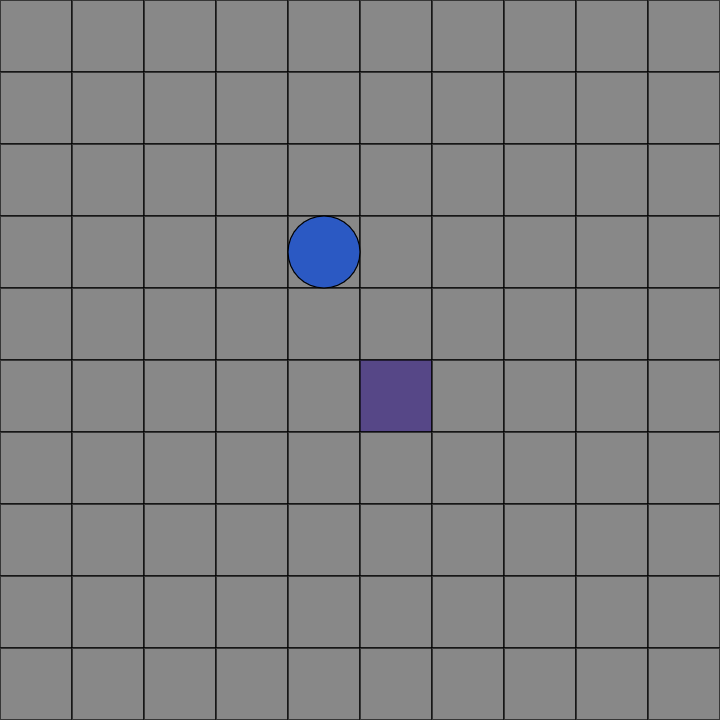
\includegraphics[scale=0.25]{app-labirint-imagine-cu-mutare}
	\caption{Reprezentarea vizual@a a labirintului dup@a o serie de ac@tiuni ale agentului}
	\label{fig:labirint-imagine-cu-mutare}
\end{figure}


\section{Simulator}

Simulatorul actioneaz@a ca o interfa@ta @intre agent @si mediul reprezentat de labirint. Acesta are rolul s@a furnizeze informa@tii c\^ atre agent, precum: codificarea curent@a a labirintului sau reprezentarea sa sub form@a de imagine; dac@a simularea este terminat@a; recompensa pentru fiecare ac@tiune luat@a.

Clasa \textbf{Simulator} este cea care define@ste structura modului de ac@tionare a simulatorului. Acesta define@ste trei func@tii principale, iar principiul lor de func@tionare este inspirat dup@a standardul definit de c\^ atre OpenAi Gym \cite{open-ai-gym-env-format}. A@sadar avem urm@atoarele func@tii:

\begin{itemize}
	\item reset - acest@a func@tie aduce mediul simulat la starea ini@tial@a (figura \ref{fig:labirint-imagine}) @si ruturnez@a aceast@a stare sub forma dorit@a (codificare sau imagine).
	\item step(ac@tiune) - aceasta transmite ac@tiunea luat@a de agent c\^ atre clasa \textbf{Board}, dup@a ac@tiunea este procesat@a, clasa \textbf{Board} transmite inapoi valoare recompensei al acelei ac@tiuni dac@a este valid@a, altfel doar anun@ta invaliditatea. Dupa preluarea rezultatului, se decide care este recompensa @si dac@a simularea s-a incheiat @in urma aceste ac@tiuni. Valorile noi starii, a recompensei @si a semnalului de terminare sunt returnate la finalul evalu@arii.
	\item actionSample - aceas@ta func@tie returneaz@a o ac@tiune aleatorie disponibil@a @in mediul simulat
\end{itemize}



\begin{lstlisting}[language=Java, caption=Definirea clasei Simulator]
class Env {
    ACTIONS = ['UP', 'DOWN', 'RIGHT', 'LEFT']
    invalidState = false
    /**
     * 
     * @param {Board} board 
     */
    constructor(board) {
        this.board = board
    }

    //
    setAgentStartPosition(pos) {
        this.board.playerDefaultPos = pos
    }

    // 
    step(action) {
        this.invalidState = !this.board.move(this.ACTIONS[action])
        return  this.board.getBoardState(), this._getReward(), this._isDone()]
    }

    //
    reset() {
        this.board.playerReset()
        return this.board.getBoardState()
    }

    //
    actionSample() {
        return Math.floor(Math.random() * this.ACTIONS.length)
    }

    //
    _getReward() {
        return (this.invalidState && !this.board.isOnExit() && -100) || this.board.getPlayerCellValue()
    }

    //
    _isDone() {
        return this.board.isOnExit() || this.invalidState
    }

    //
    clone() {
        return new Env(this.board.clone())
    }
}
\end{lstlisting}

\section{Interfa@t@a}

\section{Agent}

\begin{lstlisting}[language=Java]
class Agent {
    constructor(model) {
        /**
         * @type {tf.Sequential}
         */
        this.model = model || this.buildModel()
    }

    buildModel() {
        const model = tf.sequential()

        model.add(tf.layers.dense({ units: 10, inputShape: [10, 10], activation: 'relu' }))
        model.add(tf.layers.flatten())
        //model.add(tf.layers.dense({ units: 8, activation: 'relu' }))
        //model.add(tf.layers.dense({ units: 16, activation: 'relu' }))
        //model.add(tf.layers.dropout({ rate: 0.2 }))
        // model.add(tf.layers.dense({ units: 32, activation: 'relu' }))
        model.add(tf.layers.dropout({ rate: 0.2 }))
        model.add(tf.layers.dense({ units: 4, activation: 'linear' }))
        model.compile({ loss: 'meanSquaredError', optimizer: 'adam', metrics: ['accuracy'] })
        model.summary()
        return model
    }

    async fit(input, output) {
        await this.model.fit(tf.tensor3d([input]), output, { epochs: 5 })
    }

    predict(input) {
        return this.model.predict(tf.tensor3d([input]))
    }

    getAction(input) {
        const result = this.predict(input)
        return tf.argMax(result, 1).arraySync()[0]
    }
}
\end{lstlisting}

\section{Model de @inv@a@tare}

%% capitolul de concluzii
%%
%%

\addcontentsline{toc}{chapter}{Concluzii finale}

\markboth{\bf Concluzii finale}{\bf Concluzii finale}

\chapter*{Concluzii finale}

\markboth{\bf Concluzii finale}{\bf Concluzii finale}


\^ In aceast\u a lucrare am analizat ....
\index{concluzii}